\documentclass[a4paper,12pt]{article}
\usepackage[a4paper,top=1.3cm,bottom=2cm,left=1.5cm,right=1.5cm,marginparwidth=0.75cm]{geometry}
%%% Работа с русским языком
\usepackage{cmap}					% поиск в PDF
\usepackage{mathtext} 				% русские буквы в фомулах
\usepackage[T2A]{fontenc}			% кодировка
\usepackage[utf8]{inputenc}			% кодировка исходного текста
\usepackage[english,russian]{babel}	% локализация и переносы

\usepackage{graphicx}
\usepackage{mathtools}
\usepackage{wrapfig}
\usepackage{tabularx}
\usepackage{amssymb}
\usepackage{hyperref}
\usepackage[rgb]{xcolor}
\hypersetup{colorlinks=true,urlcolor=blue}
\setcounter{secnumdepth}{0}
%% Шрифты
\usepackage{euscript}	 % Шрифт Евклид
\usepackage{amsmath}
\usepackage{mathtools}
%%% Заголовок
\author{Tsvetkova Amelia}
\title{Лабораторная работа по общей физике}

\date{\today}
\begin{document}
\begin{titlepage}
    \newpage
    \begin{center}
    {\large МОСКОВСКИЙ ФИЗИКО-ТЕХНИЧЕСКИЙ ИНСТИТУТ (НАЦИОНАЛЬНЫЙ ИССЛЕДОВАТЕЛЬСКИЙ УНИВЕРСИТЕТ)}
    \vspace{1cm}

    {\largeФизтех-школа аэрокосмических технологий}
    \vspace{6em}
    \end{center}
    
    \vspace{1.2em}

    \begin{center}
    \Large Лабораторная работа №4.7.2 \\
    Эффект Поккельса
    \linebreak
    \end{center}
    
    \vspace{11em}
    
    \begin{flushright}
                       {\large Работу выполнила\\
                       Цветкова Амелия Антоновна\\
                       Б03-303 }
    \end{flushright}

    \vspace{\fill}

    \begin{center}
    Долгопрудный, 2025
    \end{center}

    \end{titlepage}

\paragraph{Цель работы:} исследовать интерференцию рассеянного света, прошедшего через кристалл; наблюдать изменени характера поляризации света при наложении на кристалл электрического поля. 

\paragraph{В работе используются:} гелий-неоновый лазер, поляризатор, кристалл ниобата лития, матовая пластинка, экран, источник высоковольтного переменного и постоянного напряжения, фотодиод, осциллограф, линейка.

\section{Теоретические сведения}

\subsection{Типы поляризации, основные понятия}
\textit{Плоскостью поляризации} наз. плоскость построенная на векторах ($\mathbf{E}$, $\mathbf{k}$). Плоская волна наз. \textit{линейно поляризованной}, если ориентация плоскости поляризации не меняется во времени. В \textit{естественном} свете плоскость поляризации меняется случайным образом.

Плоские электромагнитные волны являются поперечными, т.е. проекции осциллирующих электрического и магнитного полей на направление распространения такой волны равны нулю. По теореме Гаусса:
$$
\text{div}\vec{E}=\frac{\partial E_x}{\partial x}+\frac{\partial E_y}{\partial y}+\frac{\partial E_z}{\partial z}=0
$$

Из уравнения циркуляции магнитного поля:
$$
(\text{rot}\vec{H})_z=\frac{\partial H_y}{\partial x}+\frac{\partial H_x}{\partial y}+\frac{1}{c}\frac{\partial E_z}{\partial t}
$$

В итоге получаем уравнения:
$$
\left\{ 
\begin{array}{ll} 
(\text{rot}\vec{E})_y=\frac{\partial E_x}{\partial z}=-\frac{1}{c}\frac{\partial H_y}{\partial t}, \\
(\text{rot}\vec{H})_x=-\frac{\partial H_y}{\partial z}=\frac{1}{c}\frac{\partial E_x}{\partial t}\end{array}\right.
$$
и
$$
\left\{ 
\begin{array}{ll} 
(\text{rot}\vec{E})_x=\frac{\partial E_y}{\partial z}=\frac{1}{c}\frac{\partial H_x}{\partial t}, \\
(\text{rot}\vec{H})_y=\frac{\partial H_x}{\partial z}=\frac{1}{c}\frac{\partial E_y}{\partial t}\end{array}\right.
$$

В любой точке пространства концы векторов $\vec{E}$ и $\vec{H}$ в каждой из этих волн движутся по отрезкам прямых линий в плокости $(E_x, E_y)$, поэтому они \texttt{линейно поляризованными}.

Если обе описанные выше монохроматические волны распространяются одновременно, то концы векторов $\vec{E}$ и $\vec{H}$ движутся по эллипсам в плоскости $(E_x, E_y)$. Это наиболее общий тип поляризации - \texttt{эллиптическая поляризация}. Если полуоси эллипса равны, то таккую поляризацию наз. \texttt{круговой}. Свет наз. правополяризованным, если для наблюдателя, смотрящего навстречу лучу, вектор $\vec{E}$ вращается по часовой стрелке. 

Свет с круговой поляризацией можно представить как суперпозицию двух линейно поляризованных волн:
$$
\mathbf{E} = \mathbf{E}_x +\mathbf{E}_y, \quad \mathbf{E}_x = \mathbf{e}_xE_0\cos(wt), \quad \mathbf{E}_y = \mathbf{e}_yE_0\sin(wt)
$$

Монохроматические волны всегда являются так или иначе поляризованными. Если же свет квазимонохроматический (обладает нулевой шириной спектра), то возможны три случая. В первом поляризация не меняется от цуга к цугу, несмотря на сбой фазы между ними. Такой свет считается поляризованным наравне с монохроматическим. Во втором поляризации цугов меняются случайным и независимым образом. Такой свет считают неполяризованным. И в третьем случае поляризации цугов отличаются, но некоторые поляризации появляются с большей вероятностью, чем другие. Такой свет считается поляризованным частично, его можно рассматривать как смесь поляризованного и неполяризованного света.

\subsection{Получение поляризованного света}

Устройства, с помощью которых из естественного света получают поляризованный, наз. поляризаторами. Они разделяют исходный пучок на две компоненты, ортогональные по типу поляризации, одну из них пропускают, а другую поглощают или отклоняют. Действие их может быть основано на одном из четырех явлений: дихроизме, двойном лучепреломлении в кристаллах, отражении и преломлении на границе изотропных диэлектриков и поляризации при рассеянии света.

\texttt{Дихроизм} (анизотропия поглощения) - это способность вещества поглощать свет по-разному в зависимости от его поляризации. 

\texttt{Двойное лучепреломление} в анизотропнных кристаллах - результат зависимости в этих кристаллах кожффициента преломления от поляризации световой волны.

\texttt{Поляризация света при отражении и преломлении} на границе изотропного диэлетрика следует из формул Френеля.
$$
\rho_\perp=\frac{\sin^2{(\varphi-r)}}{\sin^2{(\varphi+r)}}, \quad \rho_\|=\frac{\tan^2{(\varphi-r)}}{\tan^2{(\varphi+r)}}
$$
здесь $\varphi$ - угол падения, а $r$ - угол преломления волны. Отсюда следует, что $\varphi+r=90^\circ$, т.е. угол между направлениями распространения отраженной и преломленной волн является прямым, коэффициент отражения $\rho_\|$ обращается в ноль и отраженный свет оказывается полностью поляризованным. Соотвествующий угол падения
$$
\varphi_\text{Б} =\arctan{(n)}
$$
где $n$ - коэффициент преломления среды, наз. углом \texttt{Брюстера} или углом полной поляризации. 

При \texttt{рассеянии} света на частицах пыли, молекулах газа и даже на атомах в кристаллах рассеянная волна также оказывается поляризованной, причем преимущественное направление электрических колебаний перпендикулярно падающему лучу. Интенсивность рассеянного света в газах невелика, причем согласно закон Релея она пропорциональна $1/\lambda^4$.

\subsection{Наблюдение и анализ поляризованного света. Закон Малюса}

Для анализа поляризованного света его пропускают через поляризатор, который в этом случае принято называть анализаторами. При прохождении через анализатор линейно поляризованного света интенсивность прошедшей волны пропорциональна квадрату проекции амплитуды исходной волны на разрешенное направление поляризатора, т.е.
$$
I=I_0\cos^2{\varphi},
$$
где $\varphi$ - угол между направлением электрических колебаний анализируемой волны и разрешенным направлением поляризатора. 

Для частично линейно поляризованного света вводят понятие \texttt{степени поляризации}
$$
P=\frac{I_{max}-I_{min}}{I_{max}+I_{min}},
$$
где $I_{max}$ и $I_{min}$ - соответственно максимальное и минимальное значения интенсивности света, прошедшего через анализатор при различных углах $\varphi$.

\subsection{Двойное лучепреломление}

В некоторых кристаллах потенциальные ямы, в которых находятся электроны вблизи углов решетки, не являются сферически-симметричными. При этом систему координат всегда возможно выбрать так, что для малых отклонений от положения равновесия потенциальная энергия электронов будет иметь вид 
$$
U=a_xx^2+a_yy^2+a_zz^2
$$

Если все три коэффициента $a_x, a_y, a_z$ различны, то кристалл наз. двуосным, если два коэффициента равны - одноосным. Положим $a_y=a_z=a_\perp, a_x=a_\|$. Ось $x$ при этом наз. \texttt{оптической осью кристалла}. 

\subsection{Эффект Поккельса}

\texttt{Эффектом Поккельса} наз. изменение показателя преломления света в кристалле под действием электрического поля, причем это изменение пропорционально напряженности поля. Вследствие эффекта Поккельса в кристалле либо появляется двойное лучепреломление, либо меняется его величина, либо одноосный кристалл становится двуосным.

Изменение показателя преломления кристалла под действием внешнего электрического поля происходит за счет анизотропных свойств кристаллов. Под действием постоянного электрического поля электроны смещаются в сторону того или иного иона, ппри этом меняется поляризуемость среды и связанным с ней показатель преломления. Вследвтсие линейности эффекта относительно внешнего поля $E_\text{эл}$ при изменении направления поля на противоположное должен меняться на противоположный и знак изменения показателя преломления $\Delta n$. Кристалл можно поместить между двумя скрещенными поляроидами таким образом, что в отсутствие внешнего электрического поля пропускание света системой будет равно нулю. При подаче на кристалл внешнего поля появится наведенное двулучепреломление, которое изменит поляризацию прошедшего через кристалл света, и такая система начнет пропускатаь свет. 

\begin{figure}[h]
\centering
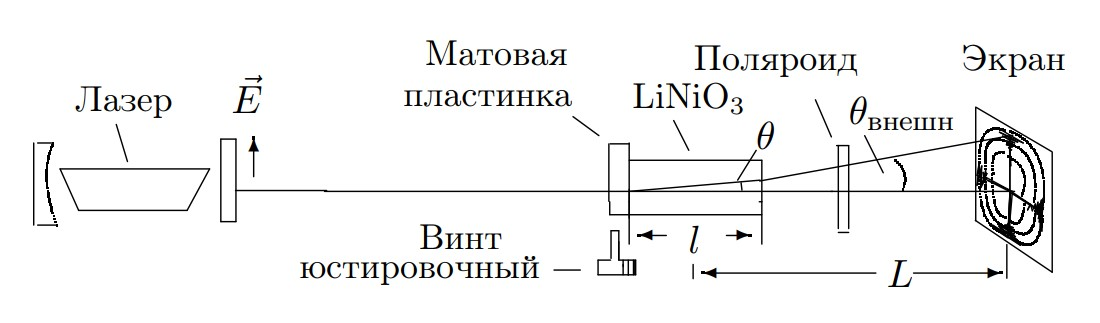
\includegraphics[width=0.8\linewidth]{img1.png}
\caption{Схема для наблюдения интефереционной картины}
\label{img1}
\end{figure}

Рассмотрим сначала кристалл в отсутствие внешнего электрического поля. Кристалл ниобата лития является одноосным кристаллом, т.е. кристаллом, оптические свойства которого обладают симметрией вращения относительно некоторого одного направления, наз. \textit{оптической осью z} кристалла. Для световой волны, вектор электрического поля $\mathbf{E}$ которой перпендикулярен оси $z$, показатель преломления равен $n_0=\sqrt{\varepsilon_{||}}$, причем $n_e<n_0$.

В общем случае, когда луч света распространяется под углом $\theta$ к оптической оси $z$, существуют два собственных значения показателя преломления $n_1$ и $n_2$: в обыкновенной волне показатель $n_1=n_0$, а в необыкновенной показатель преломления $n_2$ зависит от угла $\theta$:

\begin{equation}
    \frac{1}{n_2^2}=\frac{\cos^2{\theta}}{n_0^2}+\frac{\sin^2{\theta}}{n_e^2}
\end{equation}

Если перед кристаллом, помещенным между скрещенными поляроидами, расположить линзу или матовую пластинку, после которых лучи будут распространяться под различными углами, то на экране, расположенном за поляроидом, мы увидим темные концентрические окружности - результат интерференции обыкновенной и необыкновенной волн, точнее, проекцию их электрических полей на разрешенное направление выходного поляроида.

Разность фаз между обыкновенныой и необыкновенной волнами, приобретаемая при прохождении через кристалл длиной $l$, равна

\begin{equation}
    \Delta\varphi=\frac{2\pi}{\lambda}\cdot l \cdot (n_1-n_2)
\end{equation}

Для обыкновенного луча $n_1=n_0$ и не зависит от угла $\theta$. Для необыкновенного луча $n_2$:
$$
n_2 \approx n_0-(n_0-n_e)\theta^2
$$
Таким образом 
$$
\Delta\varphi=\frac{2\pi}{\lambda}l(n_0-n_e)\theta^2
$$

Для случая, когда разрешенное направление анализатора перпендикулярно поляризации лазерного излучения, найдем радиус темного кольца с номером $m$:
\begin{equation}
    r_m^2=\frac{\lambda}{l}\frac{(n_0L)^2}{(n_0-n_e)}m
\end{equation}

Измеряя радиусы колец, можно найти разность $(n_0-n_e)$ - двулучепреломление кристалла.

\begin{figure}[h]
\centering
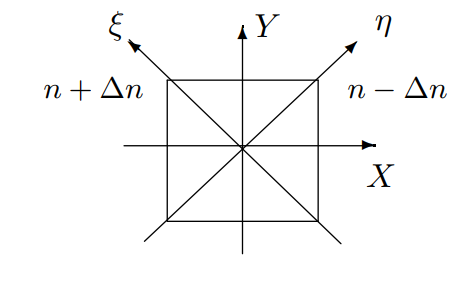
\includegraphics[width=0.6\linewidth]{img2.png}
\caption{Эффект Поккельса - появление новых главных направлений при наложении электрического поля}
\label{img2}
\end{figure}

Пусть свет на входе в кристалл поляризован вертикально, а на выходе стоит анализатор, пропускающий горизонтальную поляризацию. Разложим исходный световой вектор $E=E_0e^{i(wt-kz)}$ по осям $\xi$ и $\eta$: $E_\xi=E_\eta=E_0/\sqrt{2}$. После прохождения кристалла между векторами $E_\xi$ и $E_\eta$ появится разность фаз:
$$
\Delta\varphi=\frac{2\pi l}{\lambda}2\Delta n=\frac{4\pi}{\lambda}\frac{l}{d}AU,
$$
где $U=E_\text{эл}d$ - напряжение в кристалле, $d$ - размер кристалла в поперечном направлении. Результирующее поле анализатора:
$$
E_\text{вых}=\frac{E_0}{2}e^{i(wt-kl)}(e^{i\Delta\varphi/2}-e^{-i\Delta\varphi/2})=E_0e^{i(wt-kl)}\sin{\Big(\frac{\Delta\varphi}{2}\Big)}
$$
Интенсивность света:
\begin{equation}
    I_\text{вых}=I_0\sin^2{\Big(\frac{\Delta\varphi}{2} \Big)}=I_0\sin^2{\Big(\frac{\pi}{2}\frac{U}{U_{\lambda/2}} \Big)}
\end{equation}
Здесь $U_{\lambda/2}=\frac{\lambda}{4A}\frac{d}{l}$ - \textit{полуволновое напряжение} - имеет тот смысл, что при $U=U_{\lambda/2}$ сдвиг фаз между двумя волнами, соответствующими двум собственным поляризациям,$\Delta\varphi=\pi$, и интенсивность света на выходе анализатора достигает максимума.

\begin{equation}
    I_\text{вых}=I_0\cos^2{\Big(\frac{\pi}{2}\frac{U}{U_{\lambda/2}} \Big)}
\end{equation}

Напряжение $U_{\lambda/2}$ наз. \textit{управляющим напряжением}. Оно уменьшается с уменьшением длины волны света $\lambda$ и с увеличением отношения $\lambda/d$ кристалла. Характерная величина полуволнового напряжения в ниобате лития для видимого света составляет несколько сотен вольт.

\section{Экспериментальная установка}

\begin{figure}[h]
\centering
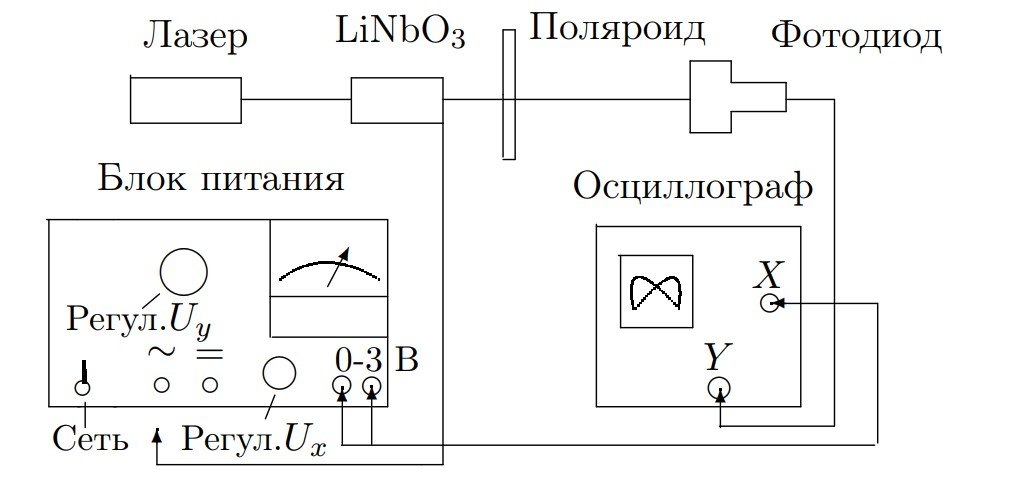
\includegraphics[width=0.8\linewidth]{img3.png}
\caption{Схема для изучения двойного лучепреломления в электрическом поле}
\label{img3}
\end{figure}

Оптическая часть установки представлена на рис.$\ref{img3}$. Свет гелий-неонового лазера, поляризованный в вертикальной плоскости, проходя сквозь матовую пластинку, рассеивается и падает на двоякопреломляющий кристалл под различными углами. Кристалл ниобата лития с размерами 3×3×26 мм вырезан вдоль оптической оси z. На экране, расположенном за скрещенным поляроидом, видна интерференционная картина.

Для $\lambda = 0,63 мкм$ (длина волны гелий-неонового лазера) в ниобате лития $n_0 = 2,29$. Убрав рассеивающую пластинку и подавая на кристалл постоянное напряжение, можно величиной напряжения влиять на поляризацию луча, вышедшего из кристалла. Заменив экран фотодиодом (Рис. 3) и подав на кристалл переменное напряжение, можно исследовать поляризацию луча с помощью осциллографа и фигур Лиссажу.

\newpage
\section{Ход работы}

\begin{enumerate}

    \item Измерим радиус темных колец $r(m)$ и расстояние $L$ от середины кристалла до экрана.

    $L=500-423=(77\pm1)$ см.
    
    \begin{table}[h!]
    \centering
    \begin{tabular}{||c|c|c|c|c|c|c|c|c||}
    \hline
        $m$ & 1 & 2 & 3 & 4 & 5 & 6 & 7 & 8 \\
        \hline
        $r_m,$см & 2.7 & 3.8 & 4.7 & 5.5 & 6.0 & 6.6 & 7.2 & 7.6 \\
        \hline
        $\sigma_{r_m}$, см & 0.1 & 0.1 & 0.1 & 0.1 & 0.1 & 0.1 & 0.1 & 0.1 \\
        \hline
        $r_m^2,\text{см}^2$ & 7.29 & 14.44 & 22.09 & 30.25 & 36.00 & 43.56 & 51.84 & 57.76 \\
        \hline 
        $\sigma_{r_m^2}, \text{см}^2=2 r_m\sigma_{r_m}$ & 0.54 & 0.76 & 0.94 & 1.10 & 1.20 & 1.32 & 1.44 & 1.52 \\
    \hline
    \end{tabular}
    \end{table}

    Построим график $r^2=f(m)$ (рис.$\ref{graph1}$). По углу наклона прямой определим двулучепреломление $(n_0-n_e)$ ниобата лития.

    \begin{figure}[h]
    \centering
    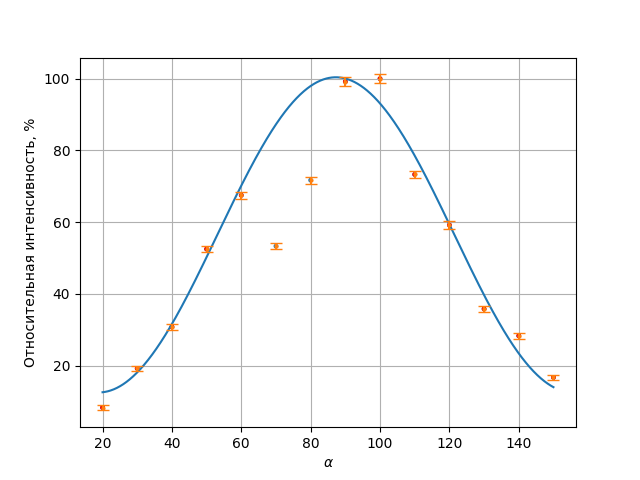
\includegraphics[width=1\linewidth]{graph1.png}
    \caption{Зависимость $r_m^2(m)$}
    \label{graph1}
    \end{figure}
    
    Величины из описания работы: $n_0=2.29,\quad l=26\text{мм}, \quad \lambda=0.63\text{мкм}$

    По коэффициенту угла наклона $k$ найдем значение для двулучепреломления $n_0 - n_e$:
    $$
    n_0-n_e=\frac{\lambda (n_0L)^2}{lk}=\frac{0.63\cdot 10^{-6}\cdot(2.29\cdot77\cdot 10^{-2})^2}{26\cdot 10^{-3}\cdot 7.27\cdot 10^{-4}}=0.104
    $$
    $$
    \sigma_{n_0-n_e} = (n_0-n_e)\sqrt{\left(\frac{\sigma_k}{k}\right)^2 + 2\left(\frac{\sigma_L}{L}\right)^2 + \left(\frac{\sigma_l}{l}\right)^2}=0.104\cdot\sqrt{\left(\frac{0.39}{7.27}\right)^2+\left(\frac{1}{84}\right)^2+\left(\frac{1}{26}\right)^2}=0.007
    $$
    
    \begin{center}
        \boxed{(n_0-n_e)=(0.104\pm0.007)(\varepsilon=6.7\%)}
    \end{center}

    табличное значение: $(n_0-n_e)=0.084$.

    \item Подключим разъем блока питания на постоянное напряжение, установим регулятор напряжения на минимальное наапряжение и включим блок питания в сеть.

    С увеличением напряжения на кристалле яркость пятна на экране увеличивается и достигает максимума при $U=U_{\lambda/2}$. При $U=2U_{\lambda/2}=U_\lambda$ яркость снова будет минимальной. Проделаем то же для параллельных поляризаций лазера и анализатора. Определим полуволновое напряжение ниобата лития.

    \begin{table}[h!]
    \centering
    \begin{tabular}{|c|c||c|c|}
         \hline
         \multicolumn{2}{|c}{Скрещенные поляризации}&\multicolumn{2}{|c|}{Параллельные поляризации}  \\ \hline\hline
         $U_{\lambda/2}$, В & $U_{\lambda}$, В & $U_{\lambda/2}$, В & $U_{\lambda}$, В \\ \hline
         480 $\pm$ 30 & 960 $\pm$ 30 & 510 $\pm$ 30 & 1020 $\pm$ 30 \\ \hline
    \end{tabular}
    \end{table}

    Среднее значение для $U_{\lambda/2} = (490 \pm 30)$ В.

    \item Подаем на кристалл напряжение $U=\frac{1}{2}U_{\lambda/2}=U_{\lambda/4}$. Поляризация на выходе кристалла круговая.

    \item Установим вместо экрана фотодиод и подключим его к $Y$-входу осциллографа. Убрав напряжение до нуля, переключаем разъем с постоянного на переменное напряжение. Отклонение луча осциллографа по оси $X$ будет пропорционально напряжению $U$ на кристалле, а по оси $Y$ - интенсивноситти прошедшего через анализатор сигнала $I_\text{вых}$.

    \item Постепенно повышая напряжение на кристалле, наблюдаем на экране осциллографа фигуры Лиссажу, соответствующие зависимости $I_\text{вых}(U)$ для скрещенных поляризаций лазера и анализатора. Слегка поворачивая кристалл, сделаем фигуру Лиссажу симметричной.

    Наблюдая за фигурой Лиссажу, определим полуволновое напряжение $U_{\lambda/2}$ как $\Delta U$, соответствующее переходу от максимума к минимуму на осциллограмме.

    $\Delta U=U_{\lambda/2}=(450\pm 30)$В

    \begin{table}[h!]
    \centering
    \begin{tabular}{|c|c|c|}
         \hline
         \multicolumn{3}{|c|}{Скрещенные поляризации} \\ \hline
         $U_{\lambda/2}$,В & $U_{\lambda}$,В & $U_{3\lambda/2}$,В  \\ \hline
         450 $\pm$ 30 & 900 $\pm$ 30 & 1350 $\pm$ 30 \\ \hline 
         \multicolumn{3}{|c|}{Параллельные поляризации} \\ \hline
         $U_{\lambda/2}$,В & $U_{\lambda}$,В & $U_{3\lambda/2}$,В  \\ \hline
         480 $\pm$ 30 & 930 $\pm$ 30 & 1380 $\pm$ 30 \\ \hline
    \end{tabular}
    \caption{Значения напряжений при измерении на переменном токе}
    \label{tab:3}
    \end{table}

    \begin{figure}[h]
		\begin{minipage}[h]{0.3\linewidth}
			\center{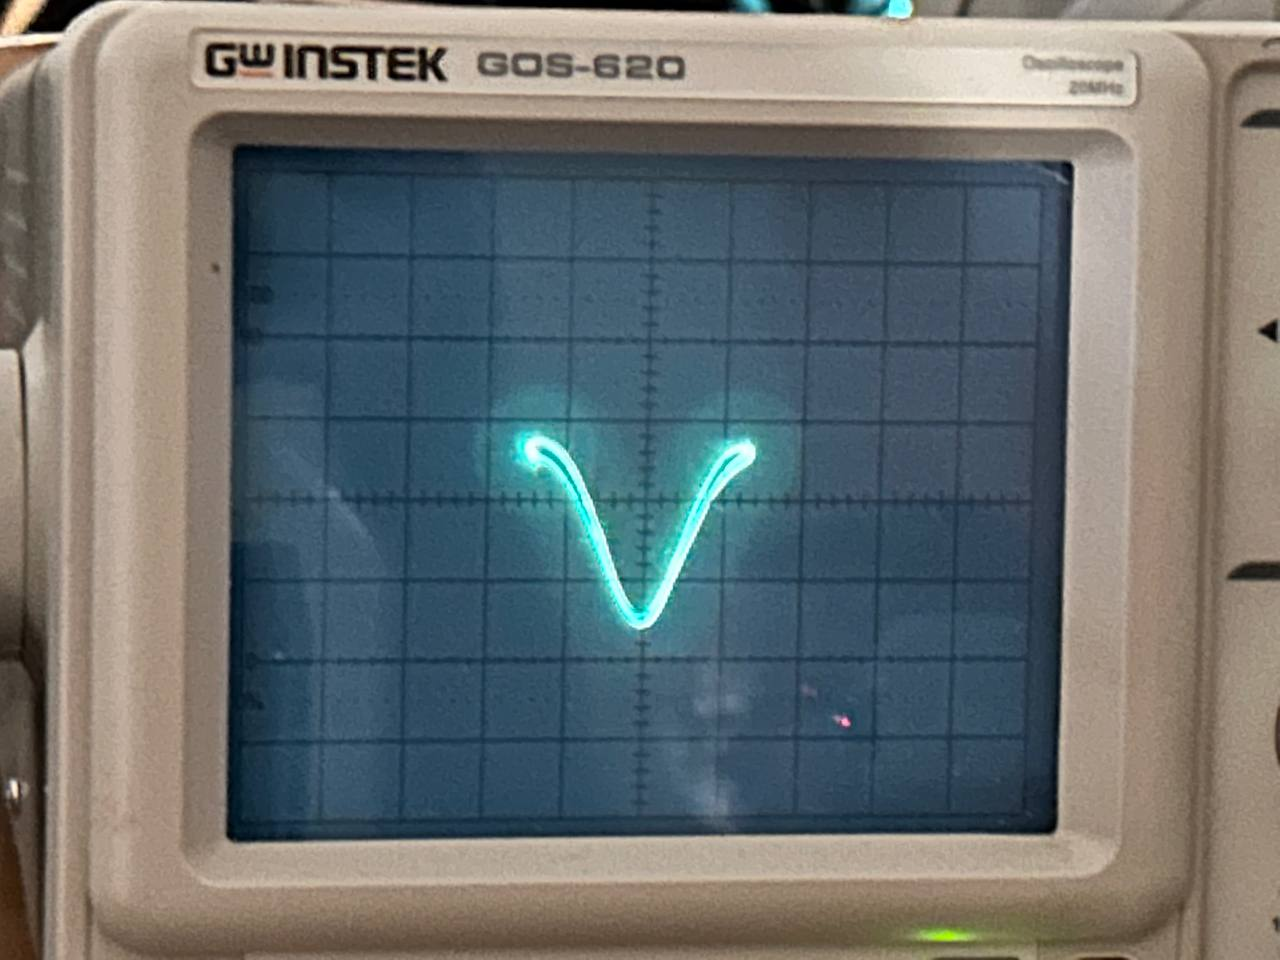
\includegraphics[width=0.9\linewidth]{img4.jpg} \\а) $U = U_{\lambda/2}$}
		\end{minipage}
		\hfill
		\begin{minipage}[h]{0.3\linewidth}
			\center{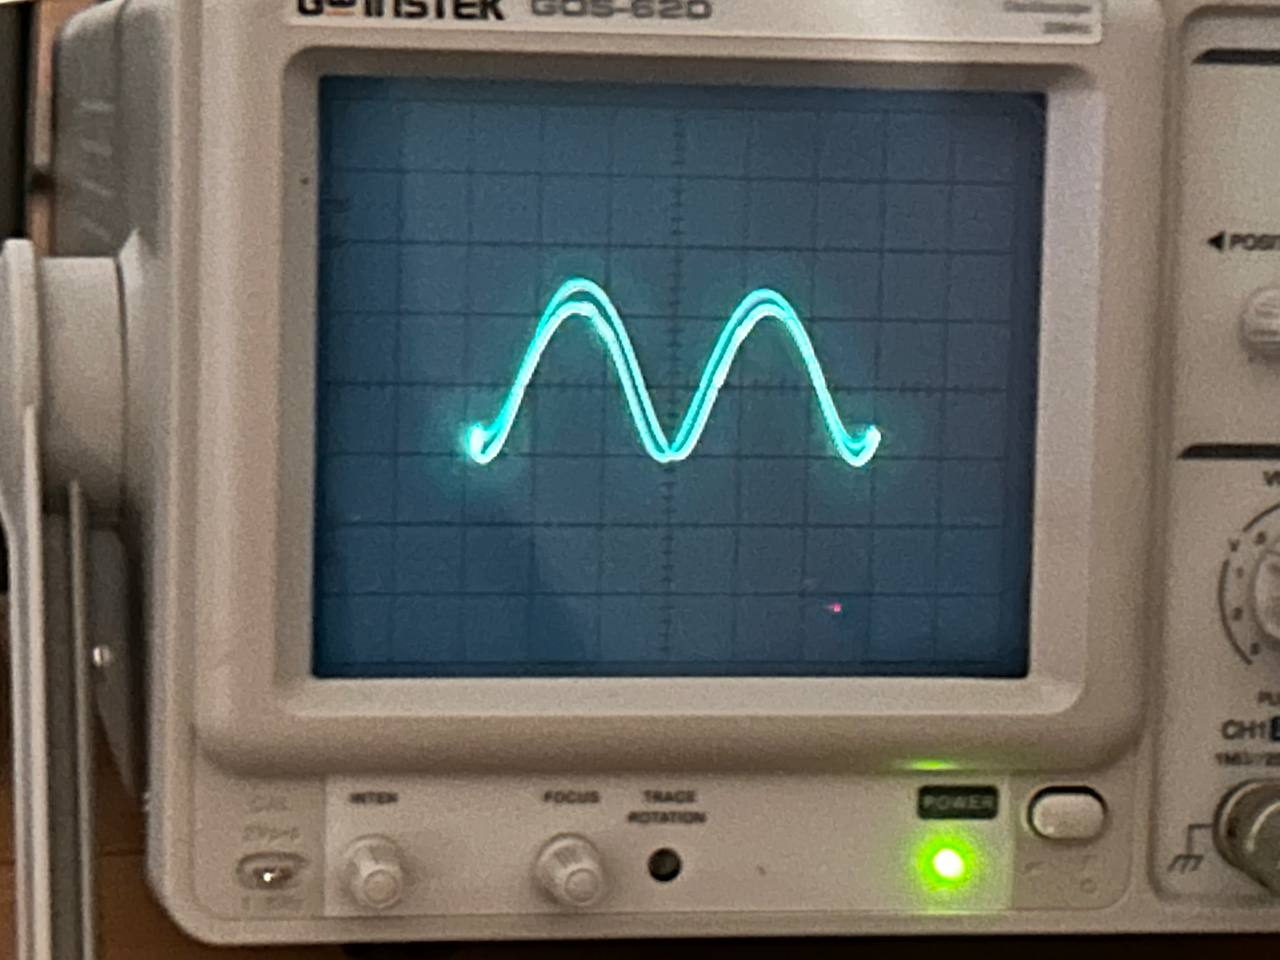
\includegraphics[width=0.9\linewidth]{img5.jpg} \\б) $U = U_{\lambda}$}
		\end{minipage}
		\hfill
		\begin{minipage}[h]{0.3\linewidth}
			\center{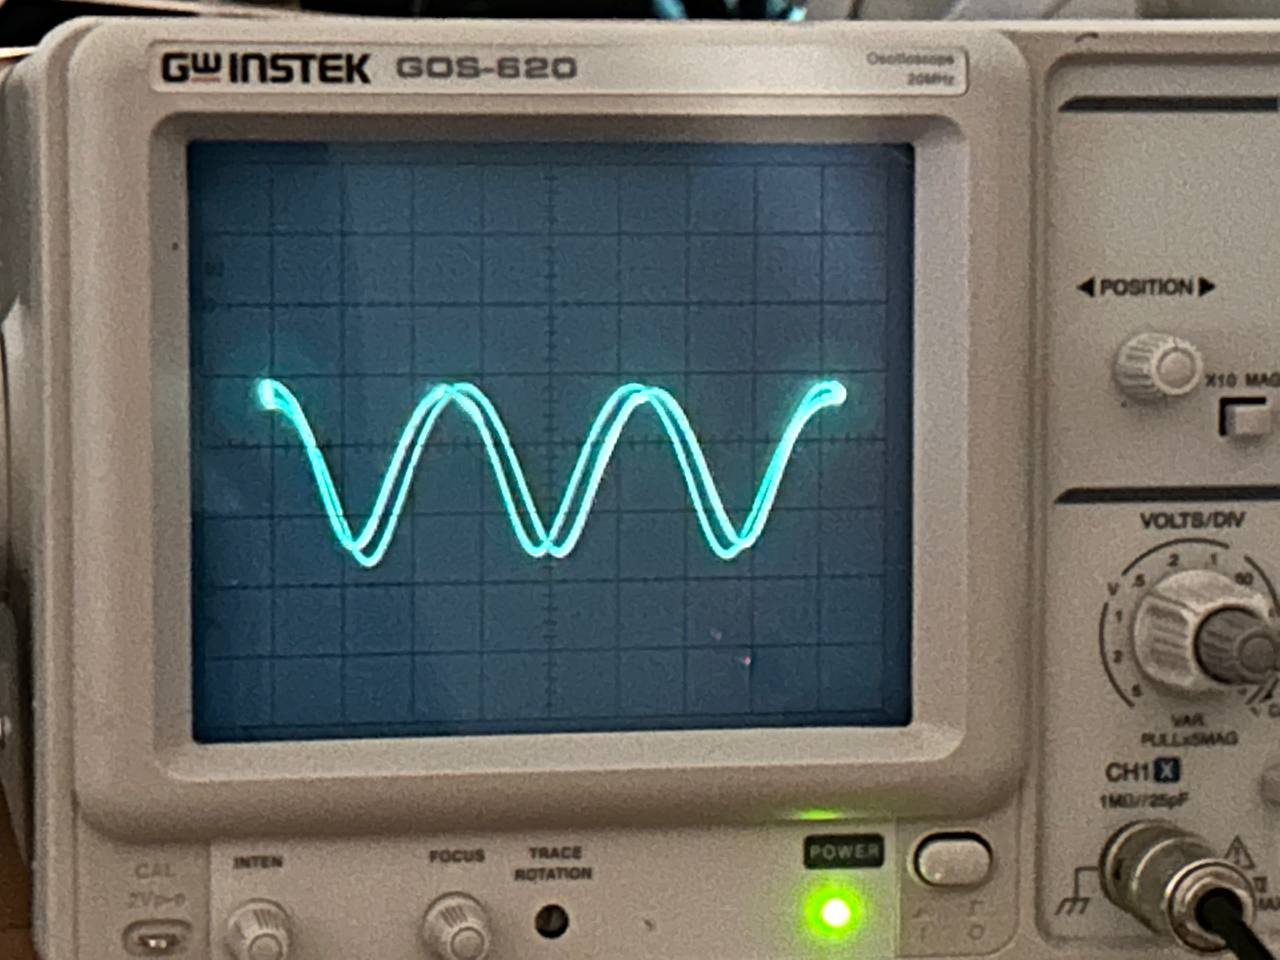
\includegraphics[width=0.9\linewidth]{img6.jpg} \\в) $U = U_{3\lambda/2}$}
		\end{minipage}
		\caption{Фигуры Лиссажу при различных амплитудах напряжения $U$}
		\label{lis}
\end{figure}

\end{enumerate}

\section{Выводы}

В ходе лабораторной работы была исследована интерференция рассеянного света, прошедшего через кристалл. По исследованию зависимости квадрата радиуса темного кольца от номера кольца был определен показатель двулучепреломления: $n_0 - n_e = 0.104 \pm 0.007$. Полученная зависимость согласуется с линейным приближением теории, рассчитанной для малых углов. При этом полученное значение близко по порядку к табличным данным для подобных кристаллов.
\par
Был исследован эффект Поккельса, в ходе наблюдения которого были определены полуволновые напряжения при постоянном и переменном токе для разных типов поляризаций (скрещенных и параллельных). В пределах погрешностей значения напряжений совпали как между разными типами поляризаций, так и между разными типами тока ($U_{\lambda/2}=(470 \pm 30)$ В.
\par
По фигурам Лиссажу, соответствующим измерениям $U_{\lambda/2}$, $U_{\lambda}$ и $U_{3\lambda/2}$, видно, что при переходе от одному напряжения к другому фаза меняется на $\pi/2$.

\end{document}
